\begin{figure}
    \centering
    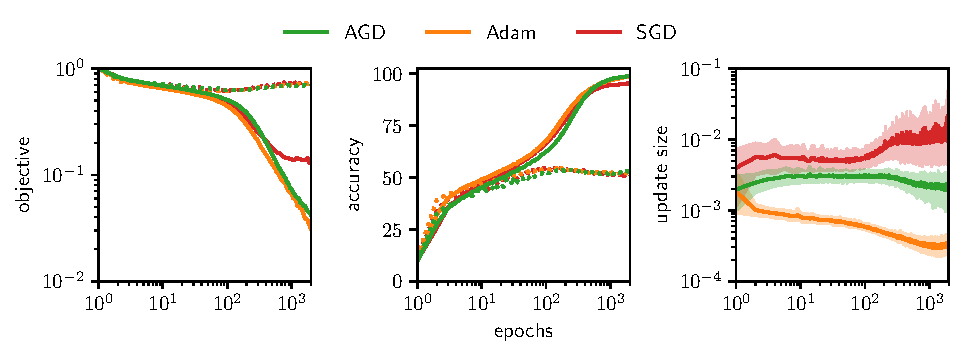
\includegraphics[width=\textwidth]{figures/pdf/plot2}
    \caption{\captiontitle{Comparing automatic gradient descent to tuned Adam and SGD.} An eight-layer fully-connected network was trained on CIFAR-10 with square loss. Dotted lines show test and solid lines show train performance.
    The \captiontitle{left panel} shows the objective value: AGD and Adam attained a smaller training objective than SGD. The \captiontitle{middle panel} shows train and test accuracies. The \captiontitle{right panel} shows the relative update size averaged over layers: $\tfrac{1}{L}\sum_{k=1}^L \norm{\Delta \mW_k}_F/\norm{\mW_k}_F$. We plot the maximum, minimum and mean over an epoch.} \label{fig:2}
\end{figure}